
%(BEGIN_QUESTION)
% Copyright 2012, Tony R. Kuphaldt, released under the Creative Commons Attribution License (v 1.0)
% This means you may do almost anything with this work of mine, so long as you give me proper credit

En stor naturgasskompressor mottar gass fra tre kilder, separerer ut væske og komprimerer gassen for rørtransport:

$$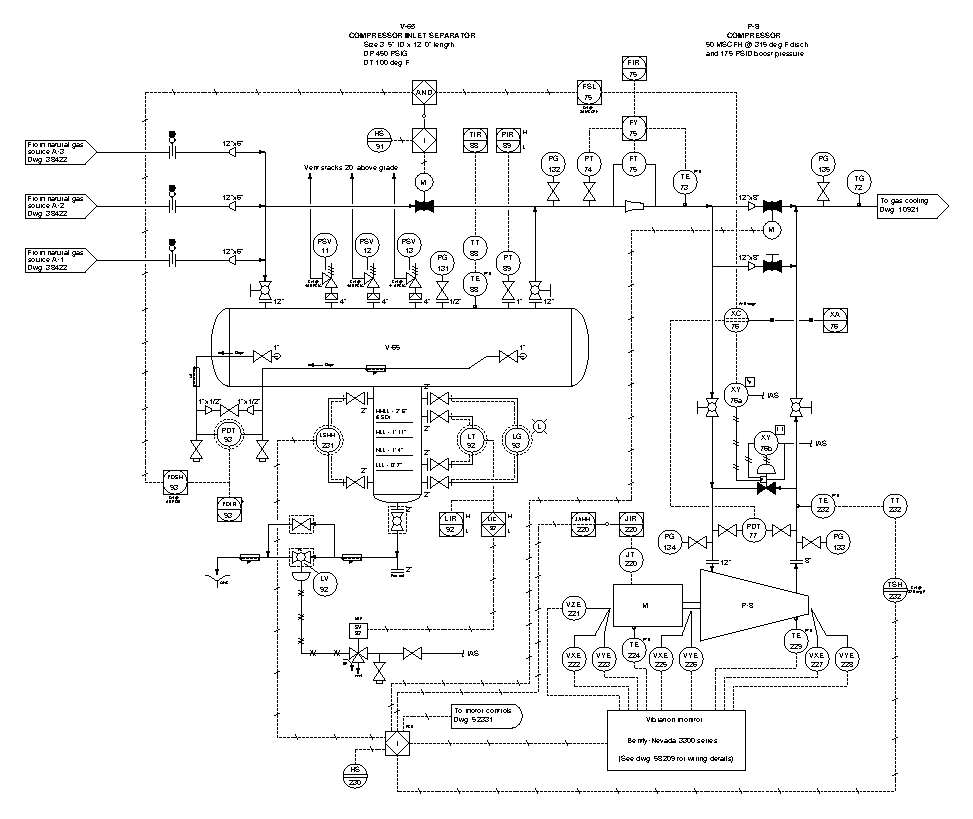
\includegraphics[width=15.5cm]{i0003rx01.eps}$$

FT-75 har vært i drift lenge, men gir ikke godt nok turndown ved drift langt under merkekapasitet. Ingeniører vurderer erstatning.

\vskip 10pt

Forklar ``turndown'' i denne sammenhengen, og hvorfor denne flowmåleren kan ha utilstrekkelig turndown.

\vskip 10pt

Foreslå ulike flowteknologier og vurder om de passer.

\underbar{file i00978}
%(END_QUESTION)





%(BEGIN_ANSWER)

Turndown er forholdet mellom minste og største flow som kan måles innen akseptabel feil. DP-baserte målere som venturi har ofte lav turndown (omtrent 4:1) på grunn av usikkerheter og ikke-lineær sammenheng mellom flow og trykkfall.

\vskip 10pt

\begin{itemize}
\item{} {\bf Fortrengning} -- ofte lite egnet for gassvolum og slitasje.
\vskip 10pt
\item{} {\bf Turbin} -- mulig, med P/T-kompensering.
\vskip 10pt
\item{} {\bf Vortex} -- mulig hvis minimumsflow er over cutoff.
\vskip 10pt
\item{} {\bf Magnetisk} -- uegnet.
\vskip 10pt
\item{} {\bf Ultralyd Doppler} -- uegnet.
\vskip 10pt
\item{} {\bf Ultralyd transit-time} -- mulig, med P/T-kompensering.
\vskip 10pt
\item{} {\bf Coriolis} -- egnet, men ofte dyr.
\vskip 10pt
\item{} {\bf Termisk masse} -- mulig hvis gassammensetning (og spesifikk varme) er stabil, ellers trengs kompensering.
\end{itemize}

 
%(END_ANSWER)





%(BEGIN_NOTES)


%INDEX% Process: gas compressor inlet separator (realistic P&ID shown)

%(END_NOTES)

